61. $\cfrac{(x-1)^3}{2x-3}\leqslant x-1\Leftrightarrow (x-1)\left(\cfrac{(x-1)^2}{2x-3}-1
ight)\leqslant0\Leftrightarrow
(x-1)\left(\cfrac{x^2-2x+1-2x+3}{2x-3}
ight)\leqslant0\Leftrightarrow\cfrac{(x-1)(x-2)^2}{2x-3}\leqslant0.$ Применив метод интервалов, найдём ответ: $x\in\left[1;\cfrac{3}{2}
ight)\cup\{2\}.$
\begin{figure}[ht!]
\center{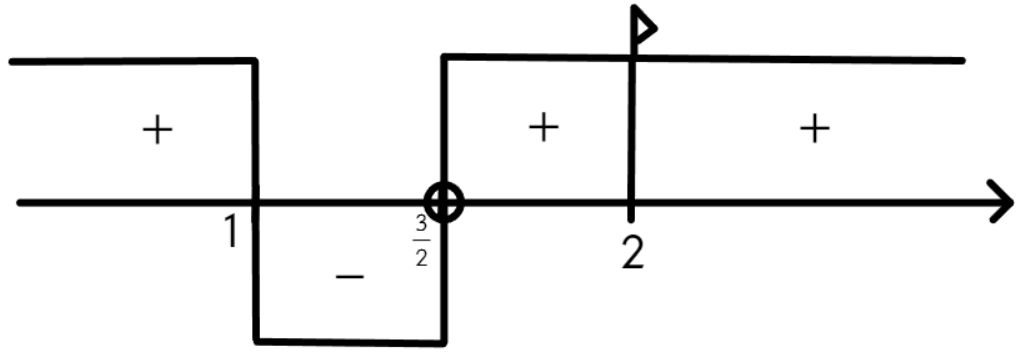
\includegraphics[scale=0.35]{ner9-61.png}}
\end{figure}\\
